%%% File-Information {{{
%%% Filename: thesis_main.tex
%%% Purpose: bachelor thesis
%%%
%%% Notes:
%%%
%%%
%%%
%%% }}}
%%%%%%%%%%%%%%%%%%%%%%%%%%%%%%%%%%%%%%%%%%%%%%%%%%%%%%%%%%%%%%%%%%%%%%%%%%%%%%%%
%%% main document {{{

\documentclass[
a4paper,     %% defines the paper size: a4paper (default), a5paper, letterpaper, ...
% twoside,     %% changes to a two-page-layout (alternatively: oneside)
% headsepline, %% add a horizontal line below the column title
% footsepline, %% add a horizontal line above the page footer
titlepage,   %% only the titlepage (using titlepage-environment) appears on the first page (alternatively: notitlepage)
% parskip,     %% insert an empty line between two paragraphs (alternatively: halfparskip, ...)
% leqno,       %% equation numbers left (instead of right)
% fleqn,       %% equation left-justified (instead of centered)
% tablecaptionabove, %% captions of tables are above the tables (alternatively: tablecaptionbelow)
14pt         %% set default font size to 12 point
]{scrartcl}  %% article, see KOMA documentation (scrguide.dvi)



%%%%%%%%%%%%%%%%%%%%%%%%%%%%%%%%%%%%%%%%%%%%%%%%%%%%%%%%%%%%%%%%%%%%%%%%%%%%%%%%
%%%
%%% packages
%%%

%%%
%%% encoding and language set
%%%

%%% fontenc, ae, aecompl: coding of characters in PDF documents
\usepackage[T1]{fontenc}
\usepackage{ae,aecompl}

%%%
%%% technical packages
%%%

%%% amsmath, amssymb, amstext: support for mathematics
\usepackage{amsmath,amssymb,amstext,amsthm}
\newtheoremstyle{mystyle}%                % Name
  {}%                                     % Space above
  {}%                                     % Space below
  {\itshape}%                                     % Body font
  {}%                                     % Indent amount
  {\bfseries}%                            % Theorem head font
  {.}%                                    % Punctuation after theorem head
  { }%                                    % Space after theorem head, ' ', or \newline
  {\thmname{#1}\thmnumber{ #2}\thmnote{ (#3)}}%                                     % Theorem head spec (can be left empty, meaning `normal')

\theoremstyle{mystyle}
\newtheorem*{definition}{Definition}
\newtheorem*{satz}{Satz}
\newtheorem*{prot}{Protokoll}
\renewcommand*{\proofname}{Beweis}
%\let\oldproofname=\proofname
%\renewcommand*{\proofname}{\rm\bf{\oldproofname}}
%\renewenvironment{proof}{{\bfseries Proof}}{}


%%% psfrag: replace PostScript fonts
\usepackage{psfrag}

%%% listings: include programming code
%\usepackage{listings}

%%% units: technical units
%\usepackage{units}

%%%
%%% layout
%%%

%%% scrpage2: KOMA heading and footer
%%% Note: if you don't use this package, please remove 
%%%       \pagestyle{scrheadings} and corresponding settings
%%%       below too.
\usepackage[automark]{scrpage2}


%%%
%%% PDF
%%%

\usepackage{ifpdf}

%%% Should be LAST usepackage-call!
%%% For docu on that, see reference on package ``hyperref''
\ifpdf%   (definitions for using pdflatex instead of latex)

  %%% graphicx: support for graphics
  \usepackage[pdftex]{graphicx}

  \pdfcompresslevel=9

  %%% hyperref (hyperlinks in PDF): for more options or more detailed
  %%%          explanations, see the documentation of the hyperref-package
  \usepackage[%
    %%% general options
    pdftex=true,      %% sets up hyperref for use with the pdftex program
    %plainpages=false, %% set it to false, if pdflatex complains: ``destination with same identifier already exists''
    %
    %%% extension options
    backref,      %% adds a backlink text to the end of each item in the bibliography
    pagebackref=false, %% if true, creates backward references as a list of page numbers in the bibliography
    colorlinks=true,   %% turn on colored links (true is better for on-screen reading, false is better for printout versions)
    %
    %%% PDF-specific display options
    bookmarks=true,          %% if true, generate PDF bookmarks (requires two passes of pdflatex)
    bookmarksopen=false,     %% if true, show all PDF bookmarks expanded
    bookmarksnumbered=false, %% if true, add the section numbers to the bookmarks
    %pdfstartpage={1},        %% determines, on which page the PDF file is opened
    pdfpagemode=None         %% None, UseOutlines (=show bookmarks), UseThumbs (show thumbnails), FullScreen
  ]{hyperref}


  %%% provide all graphics (also) in this format, so you don't have
  %%% to add the file extensions to the \includegraphics-command
  %%% and/or you don't have to distinguish between generating
  %%% dvi/ps (through latex) and pdf (through pdflatex)
  \DeclareGraphicsExtensions{.pdf}

\else %else   (definitions for using latex instead of pdflatex)

  \usepackage[dvips]{graphicx}

  \DeclareGraphicsExtensions{.eps}

  \usepackage[%
    dvips,           %% sets up hyperref for use with the dvips driver
    colorlinks=false %% better for printout version; almost every hyperref-extension is eliminated by using dvips
  ]{hyperref}

\fi


%%% sets the PDF-Information options
%%% (see fields in Acrobat Reader: ``File -> Document properties -> Summary'')
%%% Note: this method is better than as options of the hyperref-package (options are expanded correctly)
\hypersetup{
  pdftitle={Design of a Shared Parking System with special attention to security aspects}, %%
  pdfauthor={Simon Englert}, %%
  pdfsubject={}, %%
  pdfcreator={Accomplished with LaTeX2e and pdfLaTeX with hyperref-package.}, %% 
  pdfproducer={}, %%
  pdfkeywords={} %%
}


%%%%%%%%%%%%%%%%%%%%%%%%%%%%%%%%%%%%%%%%%%%%%%%%%%%%%%%%%%%%%%%%%%%%%%%%%%%%%%%%
%%%
%%% user defined commands
%%%

%%% \mygraphics{}{}{}
%% usage:   \mygraphics{width}{filename_without_extension}{caption}
%% example: \mygraphics{0.7\textwidth}{rolling_grandma}{This is my grandmother on inlinescates}
%% requires: package graphicx
%% provides: including centered pictures/graphics with a boldfaced caption below
%% 
\newcommand{\mygraphics}[3]{
  \begin{center}
    \includegraphics[width=#1, keepaspectratio=true]{#2} \\
    \textbf{#3}
  \end{center}
}

%%%%%%%%%%%%%%%%%%%%%%%%%%%%%%%%%%%%%%%%%%%%%%%%%%%%%%%%%%%%%%%%%%%%%%%%%%%%%%%%
%%%
%%% define the titlepage
%%%

% \subject{}   %% subject which appears above titlehead
% \titlehead{} %% special heading for the titlepage

%%% title
\title{Design of a Shared Parking System with special attention to security aspects}

%%% author(s)
\author{Simon Englert (2136190)}

%%% date
\date{Würzburg, am \today{}}

% \publishers{}

% \thanks{} %% use it instead of footnotes (only on titlepage)

% \dedication{} %% generates a dedication-page after titlepage


%%% uncomment following lines, if you want to:
%%% reuse the maketitle-entries for hyperref-setup
%\newcommand\org@maketitle{}
%\let\org@maketitle\maketitle
%\def\maketitle{%
%  \hypersetup{
%    pdftitle={\@title},
%    pdfauthor={\@author}
%    pdfsubject={\@subject}
%  }%
%  \org@maketitle
%}


%%%%%%%%%%%%%%%%%%%%%%%%%%%%%%%%%%%%%%%%%%%%%%%%%%%%%%%%%%%%%%%%%%%%%%%%%%%%%%%%
%%%
%%% set heading and footer
%%%

%%% scrheadings default: 
%%%      footer - middle: page number
\pagestyle{scrheadings}

%%% user specific
%%% usage:
%%% \position[heading/footer for the titlepage]{heading/footer for the rest of the document}

%%% heading - left
% \ihead[]{}

%%% heading - center
% \chead[]{}

%%% heading - right
% \ohead[]{}

%%% footer - left
% \ifoot[]{}

%%% footer - center
% \cfoot[]{}

%%% footer - right
% \ofoot[]{}



%%%%%%%%%%%%%%%%%%%%%%%%%%%%%%%%%%%%%%%%%%%%%%%%%%%%%%%%%%%%%%%%%%%%%%%%%%%%%%%%
%%%
%%% begin document
%%%

\begin{document}

% \pagenumbering{roman} %% small roman page numbers

%%% include the title
% \thispagestyle{empty}  %% no header/footer (only) on this page
 \maketitle

%%% start a new page and display the table of contents
% \newpage
 \tableofcontents

%%% start a new page and display the list of figures
% \newpage
% \listoffigures

%%% start a new page and display the list of tables
% \newpage
% \listoftables

%%% display the main document on a new page 
 \newpage

% \pagenumbering{arabic} %% normal page numbers (include it, if roman was used above)

%%%%%%%%%%%%%%%%%%%%%%%%%%%%%%%%%%%%%%%%%%%%%%%%%%%%%%%%%%%%%%%%%%%%%%%%%%%%%%%%
%%%
%%% begin main document
%%% structure: \section \subsection \subsubsection \paragraph \subparagraph
%%%

\section{Abstract}
As major cities are growing more and more, the parking situation in those cities is becoming more precarious than ever. Parking demand already exceeds the limited amount of parking spaces available, and thus people searching for a place to park generate a significant part of those cities traffic. This leads to frustration with drivers, more traffic jams, unnecessary use of petrol and further air pollution. The creation of new parking spaces is often either difficult or very expansive, which means existing parking spots have to be used more efficiently. Solutions realizing that idea to try and solve those problems are for the most part called intelligent parking systems. This thesis is focused on Shared Parking, a special kind of intelligent parking system, which opens the possibility of sharing a parking place between different people. This work features the design and implementation of such a system with special attention given to security aspects.

\section{Indrodution}

Parking in large cities is not a new problem. For decades, the search for a parking space has been something that annoys most people. Due to the ever faster growing cities in recent years, the resulting difficulties are only intensifying. The ensuing traffic for example already represents a significant part of the total traffic in city centres. According to studies around 30 percent of the daily city traffic comes from car park seekers.\cite{shoup2006cruising} In addition to the rising number of people in cities, the percentage of people who own a car continues to increase, which adds to the traffic problem. However, the traffic is not just frustrating for the drivers. The ensuing traffic jams and slow-moving traffic cause an increased amount of petrol to be burned and the air to become additionally polluted. Especially in these times, when air pollution and climate warming are becoming even more important due to Dieselgate and the capricious weather conditions, one should be looking for a solution.

The creation of new parking spaces is rarely an option. On one hand, this is often associated with high costs, on the other hand, there is usually no space for the construction of new parking spaces available in the cities. Instead, existing parking spaces must be used more effectively.

This can be done in many different ways. So-called intelligent parking systems increase the smartness of parking in different areas and therefore often lead to a more effective use of parking spaces. Intelligent parking systems are available in various forms and for most of them there are numerous scientific papers and completed projects. However, there are hardly any relevant developments for shared parking systems, which are by definition a type of intelligent parking system. A shared parking system is a trading platform on which private users can rent out and rent parking spaces. Sharing systems, such as car sharing, have become increasingly influential in recent years and are expected to continue to grow strongly. If an object is shared among different users, it is used more effectively. This applies to parking places and a shared parking system as well. Therefore, the main part of this work will be concerned with designing a shared parking system. Special attention is paid to security aspects by detailing how the system handles fraud.

First, an overview of the system is presented, in particular the system model, which depicts the different roles in a shared parking system. This is followed by functional and security requirements to be met by the design. In contrast to existing systems, the design of our system will try avoid complex hardware and manual intervention. Possible cases of fraud are described and it is noted that our system must recognize and prevent them, punish the scammers and compensate the injured party. The actual design is described in the next step. First all functional features and then the security features that determine how to deal with fraud are explained. Various modules are introduced to deal with fraud, for example enabling the rating of users or the reporting and verification of fraud. 

Subsequently, the design is evaluated on the basis of the requirements. We shall find, that the security requirements are met in most cases and that the error probability approaches 0 with increasing system size.

Once it has been shown that the design meets the requirements, an implementation, which is also part of this study, will be discussed in more detail. The design was implemented as a client-server model with Java web service running on a TomCat server and Android app for the end user.

Finally, future work will be proposed and a summary of the results will be drawn up.

\section{Related Work}
If one takes a look at existing work in the field of intelligent parking systems, he will encounter a huge chaos. There are countless scientific papers in the most diverse sub-areas of intelligent parking systems. In addition, there are numerous projects in which such systems have already been implemented. There are also some works that have set themselves the task of categorizing related work in this field. These usually serve well as a summary, but do not have uniform definitions and categorizations amongst each other. In the following we will therefore present an introduction to the topic based on these papers.

\subsection{Overview}

\subparagraph{Intelligent Parking Systems}
In general terms, Intelligent Parking Systems, also called Smart Parking Systems, are systems that try to solve the countless parking problems already mentioned while integrating 'advanced technologies and researches from various academic disciplines' \cite{idris2009car}. Thus the words intelligent or smart have different meanings depending on the time at which a system was developed \cite{fraifer2016investigation}. With further progress, especially in information technology, new opportunities are opening up and old implementations no longer seem to be 'advanced' or 'smart', but were at the time of development.

\subparagraph{Shared Parking}
Shared Parking Systems form a separate category of Intelligent Parking Systems, because they use the emerging 'shared technology' in connection with mobile devices, which are available to most people due to technological advances. Shared parking provides the framework for making purely private parking spaces available to the public by allowing them to be traded as a commodity. \cite{itdp2014shared} By sharing, parking spaces can be used more effectively and information can be distributed more easily, which reduces the aforementioned parking problems. It is taken advantage of the fact that most private parking spaces are only used by certain groups of motorists at particular times and thus remain unused for a large part of the time and that those parking times for the different groups often do not overlap.\cite{vtpi2015shared} A supermarket, for example, needs its parking spaces mainly during the day when the supermarket is opened, while a hotel needs the parking spaces at night for the overnight guests.\\

\subsection{Intelligent Parking Systems}

To give an overview we are introducing a categorization of those systems proposed by Susan Shaheen in Smart parking management field test: A bay area rapid transit (bart) district parking demonstration.\cite{shaheen2005smart} Shaheen divides intelligent parking systems into five categories.

\subparagraph{Guidance Information Systems}
Guidance Information Systems are the simplest type of intelligent parking systems. The aim of such systems is to point the car park seeker to the nearest available parking spaces. In many cities this is done by simple displays on the streets, which point to car parks and show the number of free parking spaces available in real time.

\subparagraph{Transit-Based Information Systems}
Transit-Base Information Systems are just like the previously mentioned GIS pure information systems. However, special importance is given in this case to draw attention to parking spaces and to direct to parking spaces that are linked directly to local public transport. In most cases such parking spaces are called 'Park+Ride' and allow free parking, for example. The main objective of these systems, in addition to reducing the traffic of those seeking parking, is to reduce any traffic in the city centres. The aim is to make public transport more attractive and useable in order to prevent air pollution and congestion in the cities themselves. 

\subparagraph{Smart Payment Systems}
With Smart Payment Systems operators try to minimize their maintenance costs. Setting up, emptying and repairing coin-operated machines at parking lots is often an expensive business. Operators of Smart Payment Systems therefore try to forgo using these machines. Instead, the customer pays, even contactless, with smartcards or via his own smartphone. This usually has advantages for both sides. For the customer the payment process is accelerated and he can avoid using cash and at the same time the operating costs are reduced.

\subparagraph{E-parking}
By E-parking, Shaheen referred to a special system that was under development in 2005 by a research consortium. The aim of the concept was to combine the various smart parking ideas. The system includes advanced guidance information systems, smart payments methods, reservation options and connectivity to other digital services. More generally, we consider e-parking to be systems that use all means of digitalisation to make the parking experience better and more effective for the user in all possible aspects.

\subparagraph{Automated Parking}
Automatic parking is a system in which the user simply drives the car to a general drop-off point and later picks it up from there. The system takes over the remaining transport route of the vehicle from the delivery point to the actual parking lot. Such systems also exist as manual versions, then called valet parking.

\subsection{Shared Parking}
Shaheen, like many others, pays little to or no attention to the topic of shared parking. However, according to the above definition, shared parking is a kind of intelligent parking system. Overall, there are hardly any scientific papers on this subject. There are already a few implementations of the idea, but these are either limited to certain cities or have hardly any users, which renders them useless. In addition, these systems are operated by private companies and therefore no information about the security within the system is publicly available.\\

Of the few scientific papers that exist, most are concerned with the allocation and pricing of parking spaces to potential tenants.

Shao et. al. and Yu et. al. propose in their works \cite{shao2016simple} and \cite{yu2018optimal} to use integer linear programming to maximize profits. Both studies show that their proposed strategies, in contrast to 'first-come-first-serve' or 'first-book-first-serve' strategies, lead to higher parking space utilisation and greater profits for operators of shared parking systems. Yu et. al. refer in their work only to the sharing of parking spaces of shopping malls at night. This also implies that, unlike our system, there is no fluctuation in the number of parking spaces over time which their system would not be able to handle.

Xu et. al. extend a classic matching mechanism (top trading cycles, ttc) for the parking spaces so that cash flow is allowed. They assumed that each participant owns at least one parking space and participates with this parking space in the ttc mechanism. For situations where participants are unable to rent out their own parking space or do not wish to rent another parking space, the mechanisms '(price-compatible) top trading cycles and deals (TTCD)' and 'price-compatible top trading cycles and chains (PC-TTCC)' are proposed as extensions to ttc. These allow, in addition to the already possible exchange of parking space in ttc, the flow and exchange of money within the system. These mechanisms allowed participants to save costs, but under certain circumstances negative platform's payoff would occur. \cite{xu2016private}

Xiao et. al. assign parking spaces to tenants in their work using a double auction mechanism. They present the "demander competition padding method (DC-PM)" auction mechanism based on a slot allocation rule and a transaction payment rule. Both demanders and bidders place their bids by specifying the parking price and time and the mechanism determines the allocation of the parking spaces. Since this mechanism can lead to distorted social welfare, a "modified demander competition padding method (MDC-PM)" auction mechanism is also proposed, which is however inferior to the first mechanism in terms of its usefulness for the participants. They show that both mechanism "can realize asymptotic efficiency as both demanders and suppliers approach infinity", but do not take the spatial requirements of the participants into account during the allocation process. \cite{xiao2018shared}

Zhang et. al. try to improve the competitiveness of shared parking lot providers compared to traditional parking lots. They use the Hotteling model to compare the product differentiation of the two parking systems and use equilibrium analyses to evaluate the parking prices. \cite{zhang2019pricing}

In all these papers, the utilisation of parking spaces or the social welfare in the system improves compared to the 'first-book-first-serve' mechanism, but the systems do not provide the user with the same level of transparency. In our shared parking system, users should be able to see exactly which parking spaces are available, choose from them and be sure to be able to use the selected parking space. This can only be implemented with 'first-book-first-serve' and the systems mentioned above are not able to provide this functionality.\\

In addition to parking space allocation through a matching mechanism, Kim et al. propose an infrastructure to help drivers find the optimal parking space. The infrastructure consists of Road Side Units (RSUs), which communicate with the cars of parking seekers and Fog servers, which monitor the availability of each parking lot. RSUs communicate directly with Fog servers in their vicinity and with each other through a Roadside Cloud. Users can now make a request while driving, which is then accepted by the RSUs. Through communication between the RSUs and with the Fog Servers, a matching problem with all car park seekers is established, solved and the allocation of parking spaces is sent back to the vehicles through the RSUs. \cite{Kim2015ASP}

The big problem for this system are the expensive implementation and maintenance costs which arise because a lot of hardware and sensors have to be installed. The operator has to provide the RSUs, the Fog Server, sensors for each parking spot and the Roadside Cloud and every participant requires appropriate channels of communication on his car to connect to the RSUs. Our system, on the other hand, will do without expensive hardware to reduce maintenance costs and enable anyone to participate.\\


A number of shared parking platforms have already been implemented, but in very few cases they have become established. Internationally, for example, justpark.com or mobypark.com offer this service, in Germany there are providers like parkplace.de and parklist.de. All these platforms offer private individuals the opportunity to offer their own parking spaces, but the supply is very limited.

At parkinglist.de, even in large German cities such as Munich, there is almost exclusively only information about public car parks or offers for monthly rented parking spaces from car park operators, but hardly any private offers.

At parkplace.de there is also only a small number of almost exclusively long-term parking spaces available. Moreover, this platform does not offer the possibility to automatically perform payments. Instead, payment-specific matters have to be agreed on with the landlord separately.

At justpark.com, which originates from England, there are almost exclusively public parking garages available in London, for example. However, many car parks also offer the possibility of making reservations.

At mobypark.com you can find some listings from private persons. However, Mobypark is not widespread and is only really represented in a few cities, such as Amsterdam and Paris.

However, none of the providers discloses information on how they can protect their systems and users from fraud and how they generally deal with fraud. This is presumably because, as Mobypark itself reports on its website, parking spaces are hardly rented for short periods of time like a few hours, but mainly for longer periods (several days to several months). In addition, most of the rented parking spaces are not publicly accessible and key cards or the like must be exchanged prior to and at the end of the rental process. These conditions already lead to a reduction of fraud possibilities. In our application, however, it should also be possible to rent freely accessible parking spaces, even for short periods of time. This creates new opportunities for fraud, which, unlike in the scientific papers mentioned above, we will address in this paper.

\section{System Model and Requirements}
Now that an overview of the topic has been provided, the next part will deal with a basic system model and the requirements that will be imposed on the design. The system model gives an overview of the different parties that exist in our shared parking model and their relationships with each other. The subsequent requirement analysis is divided into functional and security requirements. Special attention is paid to ensuring that the design is secure. For us security requirements do not only refer to standard security aspects such as encryption, user authentication and authentification, but in particular to the goal of designing our shared parking system in a way that it has the ability to handle fraud independently. The aim of those aspects is to prevent and punish individual users from scamming other users or the system. Various forms and examples of such fraud will be explained in more detail below. The design set up in the later part of the work will adhere to these requirements. We will now start of with a High-level Overview of the Shared Parking System.

\subsection{High-level Overview}
This section gives a high-level overview of the shared parking system to be designed and deals with the basic capabilities of the system. The shared parking system adheres to the definition supplied at the beginning. It offers a platform for an online marketplace where both private and business users can rent and lease parking spaces. End users have the possibility to install an app and participate in the marketplace via their smartphone. This also clarifies the basic capabilities of the system. Every user can offer his own parking spaces for specified periods of time on the platform for rent. Users can also view other users' listings, choose from them and rent those parking spaces. In this system, particular importance is attached to handling fraud. The subsequent requirements define the exact framework under which the design was developed. 

\subsection{System Model}
The following system model, which is depicted in figure xy, shows the various parties in our shared parking system. On the one hand, there is exactly one operator or service provider. This service provider is responsible for the implementation of the design, operating the system and making the systems services available to the users. The users are those who utilize the system. They can be divided into two roles, whereby a user can be part of both roles at different points in time. On the one hand, there are landlords who own a private parking space and want to rent it out over a certain period of time. On the other hand, there are tenants who are looking for a free parking space to rent for a specific time period. In the course of the thesis, further roles are assigned to the users, which are always explained as soon as they are needed.\\

To-Do: Figure of system model

\subsection{Functional Requirements}
The following will cover the main functional requirements in detail.
\subparagraph{Basic Hardware} Neither the operator nor the user should need any additional and expensive hardware. For getting the system to work the user just needs a off-the-shelf smartphone and the operator only needs to provide enough computational power to get the server running. There will be no sensors installed at the parking spots, no additional hardware used for confirming parking time or the likes of that.
\subparagraph{Intuitiveness} The implementation of the design should be intuitive to use. First time users should be able to book or rent a parking space within minutes. Tasks such as user authentication should not be to complex or time-consuming.
\subparagraph{Neutral Balance} The operator or the system has different costs and revenues. Thus, the operator can either make a profit or lose money. We impose the condition on the system that in the long run, the revenues at least cover or even exceed the costs. This means that there may be time spans in which the costs are greater than the revenues, but if you take a look at the system in the long term, the revenues must surpass the costs.
\subparagraph{Automatic Processing} Where possible, the system should be prevented from requiring manual intervention. All basic use cases should be able to run automatically by the system. The system may only request manual intervention in exceptional cases. On the one hand this should lead to a fast processing of all inquiries and on the other hand reduce the costs arising from manual work.
\subparagraph{More to come}

There are also areas that do not place any functional requirements. There are aspects to which no special significance is attached in this work. This includes, for example, all legal matters. On the one hand, this work is in the field of computer science and the author does not have the fundamental knowledge to evaluate and judge legal matters. On the other hand, the legal aspect of a shared parking system involves many and various legal factors, which would exceed the scope of this work. Nevertheless, attention was paid during the design to carry out as little legal interference as possible in order to avoid legal difficulties during the implementation.

\subsection{Security Requirements}
The following will cover the main security requirements in detail.
On the one hand, requirements are made on information technology security and on the other hand, requirements are mode on how to deal with fraud in the shared parking system. When we talk about fraud, we mean a user's ability to scam other users or the system using its normal functionality in order to gain a profit. In many cases, this has a negative impact on other users. There are numerous possibilities for fraud in the system, some of which are mentioned as follows. We will categorise all fraud cases into three different classes. From now on, we refer to a user who commits fraud as a scammer. Users who are affected by fraud in a negative way will be called injured or injured party. \\

The first class of fraud cases are those in which a tenant has booked a parking space, but  it is not available when he arrives. There could be different possibilities as to why the parking space is not available, examples of which are the following.
\begin{itemize}
\item Scammer parks in a car park, which he has not booked and thus without paying the owner.
\item Tenant overstays his booked parking time.
\item Landlord rents out a parking space, but remains on it himself.
\item Landlord offers the same parking space multiple times.
\item Landlord offers a parking space that does not exist.
\end{itemize}
As we will see later, Class 1 cases can be handled by our system without manual intervention. \\

We will introduce various modules, such as a report module, to deal with these cases. While these modules will help to deal with Class 1 fraud, they create the opportunity for a new series of fraud cases. These new fraud cases, which we will group into Class 2, try to take advantage of the methods we have introduced to deal with Class 1 fraud. Examples are the ones below.
\begin{itemize}
\item User tries to impose costs on to the system by doing false reports.
\item Scammer pretends to be the injured party.
\item Scammer accuses another user of fraud.
\end{itemize}
We shall see that Class 2 cases can also be solved without manual intervention by expanding our modules. \\

While the first two classes cover the main and most frequent cases of fraud, there are others. Class 3 cases differ from the other classes in that it will not be possible to solve them without manual intervention. These are exceptional cases that occur only in low frequency. Examples are given below.
\begin{itemize}
\item Landlord rents out parking spaces that they do not own themselves.
\item Tenant cancels booking of parking space without paying.
\end{itemize}

The system must be able to handle all these cases of fraud mentioned above successfully. In the following we will define what we mean by 'successful handling'. We therefore set requirements that must be met for the various cases of fraud.
\subparagraph{Fraud Prevention} The design of the system should be such that fraud is fundamentally prevented. If this is not possible in all cases, it should be ensured that it is not worth the effort for the scammer or that scammers are quickly discovered. This is where the second point comes into play.
\subparagraph{Fraud Detection} The system should be able to detect fraud. This includes, on the one hand, the simple recognition of fraud and, on the other hand, the ability to correctly identify the scammer. The later is particularly important for the next point.
\subparagraph{Fraud Punishment} The design should be such that a scammer can be punished by the system. After a scammer is detected, the system should always be able to penalize him. Punishment can also support the first requirement by acting as a deterrent for fraud.
\subparagraph{Fraud Compensation} Finally, the system should be able to compensate an injured party. If injured are compensated, there is no need for genuine users to worry about fraud and thus enhances the attractiveness of the system.\\

There are also areas that do not place any special requirements on security. Even without a shared parking system, attacks on the private parking infrastructure are possible. One person can for example park their car in another person's private car park. The injured party has two options, both of which can have strong disadvantages for him. He could call the towing service, hope that the scammer has not left by its arriving time or he will have to bear the expensive towing fees himself. The other option is to do nothing and look for a new parking space for yourself. Such problems, which are already present, do not need to be solved. However, it can be seen as a added bonus to prevent such problems with good design choices for the shared parking system.


\section{Design}
With the requirements being defined, the next part is devoted to the actual design. As with the requirements, we will first have a look at the functional features before dealing with fraud.

\subsection{Functional features}
The functional features will be presented as use cases.
\subparagraph{User registration} The registration process is rather simple. A user registers by entering his e-mail address, his first and last name and a password. After confirming the data, a mail is sent to the specified address, in which the user must verify whether it actually is his address.

From this point on he can log into the system at any time using his mail address and password.

\subparagraph{Balance system} Each user has a credit balance that can be charged and paid out using standard payment options. Various events, such as renting or hiring out a parking space, lead to an increase or decrease to the credit balance. The precise calculation of the credit is defined below for the individual events. If a user's balance is negative, they will no longer be able to use the system. His credit must be recharged before his next action.

\subparagraph{Parking Space management} Before you can rent a parking space, you have to register it in the system. To do this, enter the address and select the exact location on a map so that the coordinates (latitude and longitude) of the car park can be stored in the system. In addition to registration, these parking spaces can also be removed.

\subparagraph{Renting out a parking space} If a user wants to rent out a parking space, he inserts an offer. He selects one of his parking spaces, specifies the time at which the parking space is available and the price that the rental will cost per hour.

\subparagraph{Renting a parking space} If a user wants to rent a parking space, first a map is presented. There his location can be displayed or he can search for a city/address to be centred. All currently available parking spaces are displayed on this map. In addition to the location, the user can specify the time at which he wishes to book the parking space. If he does, only parking spaces that are available for the entire time period are displayed.

\subparagraph{More to come}
  
\subsection{Security features}
In order to prevent fraud different modules are introduced. There is a rating module, reporting module and a verification module, all of which are explained below. These modules work together and provide information for a reputation module that assesses the trustworthiness of each user. At the end of this section an example is given on how the design utilizes those systems to handle fraud.

\subsubsection{Rating Module} The design of the shared parking system includes an rating module, allowing users to rate each other. After each rental agreement has been concluded, both tenants and landlords have the opportunity to give the other party a rating. The rating consists on the one hand of a points/star rating between 1 and 5, and on the other hand of a rating text. The user should share his experiences made with the other party and evaluate how satisfied the agreement went for him. The ratings each user received are displayed on his user page and in all of his offers. The rating system is designed to help eliminate scammers and encourage users to be as friendly and courteous as possible.

\subsubsection{Reporting Module} The next important component is the reporting module. Whenever a user detects a rule violation by another user, he has the possibility to report it. A distinction is made between the reporting user, the reported user and the inspectors, who will be explained in the section 'Verification Module' later.

Firstly, there is the possibility of reporting a violation that occurs during a rental contract. On the overview page of the contract, you can choose from various reporting reasons, all of which refer to this contract. If the user finds a suitable violation from the list, he selects it and the system can respond to it without manual intervention. For example, tenants always have the option "The rented parking space is occupied by another vehicle", in which the license plate of the car, which occupies the parking space, is also provided. In a similar way, there is the option "Tenant has overrun parking time". for landlords. For all reasons that are not explicitly mentioned, meaning that the system cannot resolve them automatically, there is a general reporting function that requires manual intervention from the provider.

If the system receives a report, it can be sure that it is always a case of fraud. Either the user reports a real fraud case, which in this case has to be fraud class 1, or it is a false report from the user, which he expects to benefit from. This would again be a case of fraud, which can be classified in fraud class 2. The system must therefore first check the truth of the message. The verification system exists for this purpose and is explained below. This system now checks whether the report was given truthfully and acts accordingly. How exactly the system acts is explained in detail in the section 'Sanctioning and Compensation'.

\subsubsection{Verification Module} Another important security tool is the verification module. It allows the system to check whether a rule violation has actually been committed. Rule violations that can be verified in this way are those of fraud class 1. If such a situation occurs and another user cannot occupy his legally entitled parking space, he will report it to the system. Since the report may also be false, the system must verify it. For this purpose, other users are called upon to go to this place and to name the license plate of the car in the parking lot as well. The truth of the report can be verified by comparing these results. The verifying users will receive a bonus on their balance for their service.

The module works in several steps. After a message is received, potential inspectors are selected. They confirm that they will verify the report. Afterwards, they verify the report and the system evaluates the results. \\

Since the location of the inspectors must be taken into account when selecting them, users have the option of deciding whether they want to participate in the verification system or not. There are two ways for all participating users to provide the system with location information. 
\begin{itemize}
\item The user allows the app to retrieve GPS data from the mobile device. The GPS data is only collected if a report needs to be verified. Directly after viewing the data, it is calculated whether the user is in the area, and the GPS data is deleted again.
\item The user selects an area on a map in which he wants to verify reports. GPS data is not necessary.
\end{itemize}

A list is created of all users that are eligible for verification. This list will now be sorted so that the users who are most suitable are at the top and users who are less suitable are at the bottom. Suitability is determined using a 'connection' score, which is calculated for all available inspector. This score indicates the independence between the inspector and the reporting and the reported user. A low score is a sign of great independence. 'connection' is a score, which represents the number of common events between the inspector and the reporting user plus the number of common events between the inspector and the reported user in the last six months. The following events increase the score between user 1 and 2 by a single point.
\begin{itemize}
\item User 1 books a parking space with user 2.
\item User 1 reports user 2.
\item User 1 verifies a report from user 2.
\end{itemize}

Now the users from the list are asked whether they can verify this case. This request is not sent to all users at the same time. Based on the reputations score (see below) it is determined how many inspectors n are needed to solve the case and requests are sent to the first n*3 inspectors of the list.\\

The selected users will receive a notification on their smartphone indicating the location of the case for review. They then confirm or reject whether they want to and can perform the verification within the next 30 minutes. If a user refuses or does not respond within 15 minutes, he will be removed from the list and the next user not yet contacted will receive a request.\\

As soon as a user has accepted the request, he will receive exact information about the parking space. He then moves to the inspection point and states whether this parking space exists and which car is parked on it according to the license plate.

\subsubsection{Reputation Module} The last part of the security features is the reputation module. It stores a hidden value for each user, which is updated using the other security modules. The value indicates the trustworthiness of a user. It is needed because the system cannot always decide with certainty who is right in the event of a conflict. For example, if a scammer departs his unpaid parking space until the inspectors arrive, it cannot be decided whether it was a false report or whether the scammer has actually occupied the parking space. In such cases, this value is used to make a decision. \\

The value will always be one of five options. 'neutral' means that there is not enough information about the user to form a judgment. 'untrustworthy' means that the user has often been noticed negatively and his credibility is therefore in question. The system displays an even lower credibility towards the user with the value 'very untrustworthy'. In contrast, 'trustworthy' and 'very trustworthy' represent a high level of credibility acquired by the user. \\

All other modules already mentioned are included in the calculation of the value. All events of a user are divided into positive, neutral and negative events and thus influence the reputation value. If a user is rated well (4 or 5 stars) or serves as an inspector to successfully solve a case, his score can be increased. If, on the other hand, he receives a bad rating (1 or 2 stars), is reported and convicted as a scammer, gives a false report or deceives the system as an inspector, his score can be reduced. The exact calculation works as follows: \\

\subparagraph{Neutral} Users with five or less events are always rated 'neutral'.
\subparagraph{Untrustworthy} Users with a minimum of 5 negative events among their last 20 are rated 'untrustworthy'. If less than 20 events (but more than 5) exist, users are classified as 'untrustworthy' if at least a quarter of the events are negative.
\subparagraph{Very Untrustworthy} Users with a minimum of 10 negative events among their last 20 are rated 'untrustworthy'. If less than 20 events (but more than 5) exist, users are classified as 'untrustworthy' if at least half of the events are negative.
\subparagraph{Trustworthy} Users among whose last 20 events are less than 5 negative are rated 'trustworthy'. If less than 20 events (but more than 5) exist, users are classified as 'trustworthy' if less than a quarter of the events are negative.
\subparagraph{Very Trustworthy} Users with at least 20 events, of which a maximum of 2 are negative are rated 'very trustworthy'.

\subsubsection{Deciding who the scammer} After receiving a report, the system must first decide who the real offender is: the reported user or the reporting user. For this purpose, the order is passed on to the verification module. The verification module sends a chronologically sorted series of verifications as a response. Once it has been received, the system can make a decision. The following options are possible:

\subparagraph{Complete consistency} Complete consistency is the simplest of the scenarios. To declare a series of verifications as completely consistent, the first verification must always correspond to the given report. If all other inspectors also report the same incident, the system decides to acknowledge the reported user as guilty. However, complete consistency also exists if the reported event changes over the period of time, but remains logical. The verfications that follow after the first one must match over time. For example, the scammer could leave the parking lot after the first inspector. If then all the other inspectors report that the parking lot is free, it is still a consistent series.

\subparagraph{Inspector consistency} Another possibility is that although all inspectors report the same, those verfications do not match the report received. This could be because the report was a false report or because the situation changed by the time the first inspector came. The system must resolve this conflict, as described in the next section 'Resolving a Conflict'.

\subparagraph{Inconsistency} The last possibility is that some verifications contradict each other over the temporal course. If inspector 1 and 3 have seen the same car in the parking lot, it is very unlikely that the parking lot was free at the time inspector 2 has checked it. If such inconsistencies are found, they are removed from the series and attributed to the inspector as a negative event. Furthermore, he does not receive any credit for his verification service. After the series has been cleaned up, the system will once again check what type of series it is.

\subsubsection{Resolving a Conflict} If a conflict occurs, it must be resolved. This is done using the reputation system. For this purpose, the reputation values of both parties to the conflict are compared. The result of a conflict is either undecided or a victory for one party and thus a defeat for the other. The system proceeds in the following order.

\begin{enumerate}
\item If both parties of the conflict have the same reputation value, it is considered as undecided.
\item If one of the two parties is classified as 'very untrustworthy', it is considered the loser of the conflict.
\item If either party is classified as 'very trustworthy', it is considered the winner of the conflict, unless the other party is 'neutral'. In which case, the conflict is considered as undecided.
\item In all other cases in which at least one of the two parties is classified as 'neutral', the conflict is considered as undecided.
\item The last remaining case is between a party classified as 'trustworthy' and a party classified as 'untrustworthy'. The party classified as 'trustworthy' is considered the winner of the conflict.
\end{enumerate}

\subsubsection{Dealing with fraud} With these basic systems it is now possible for the system to punish scammers and compensate the injured parties. 

After a report has been received, the reporting user will first be provided with a new parking space, regardless of whether it later turns out that he was in fact the fraudster. For this purpose, the system selects the nearest parking space available for the entire duration of the reservation of the original parking space. The system now books this parking space for the reporting user, takes over the costs, and sends the information about it to his smartphone. The System however, will not pay the price which is officially offered for the replacement parking space, but will instead pay the average price of parking spaces in the area. This is calculated as the average price of all bookings of the last x months in a maximum distance of y kilometers. On registration, all users agree to make their parking space available as a replacement parking space for the average parking fee, if required. The reporting user can now use the replacement parking space and the owner of the replacement parking space will be fairly remunerated.

After a replacement parking space has been provided, the already explained modules and methods are used to determine who the scammer is.

If a definite perpetrator is identified, he will be punished. The punishment of fraudsters is primarily enforced by a fine. The penalty will be deducted from his credit balance. This penalty will also be used to cover the costs of the fraud. Costs arise on the one hand when compensating the injured party and on the other hand when paying the inspectors. The penalty is calculated from the sum of the inspectors' credit bonuses and the remuneration of the landlord of the replacement car park. Thus there are no costs for the system when the offender is successfully identified. 

However, if it is not clearly determined who the fraudster is, the system must bear the costs itself. We will show later that this occurs only in a small number of cases.

\subsubsection{Example}
Figure \ref{img:example-grafik} on page \pageref{img:example-grafik} shows fraud within the system and how to deal with it. The procedure is explained in more detail below.\\

User 1 has booked a parking space in advance that belongs to user 2. He's already paid him. However, when he arrives to occupy the car space, he realizes that another user (user 3) is already blocking the parking place. He then uses the reporting system to report user 3 with his license plate. The system receives the message and then assigns other independent users with the task of checking the message. In the meantime, user 1 will be provided with a new parking space (parking space of user 4). He can use it free of charge for parking the same duration as his originally booked spot. After verifying the violation made by user 3, the system now collects the fine from him and pays user 4 for his parking space and the other users for verifying the report.\\

\begin{figure}
	\centering
	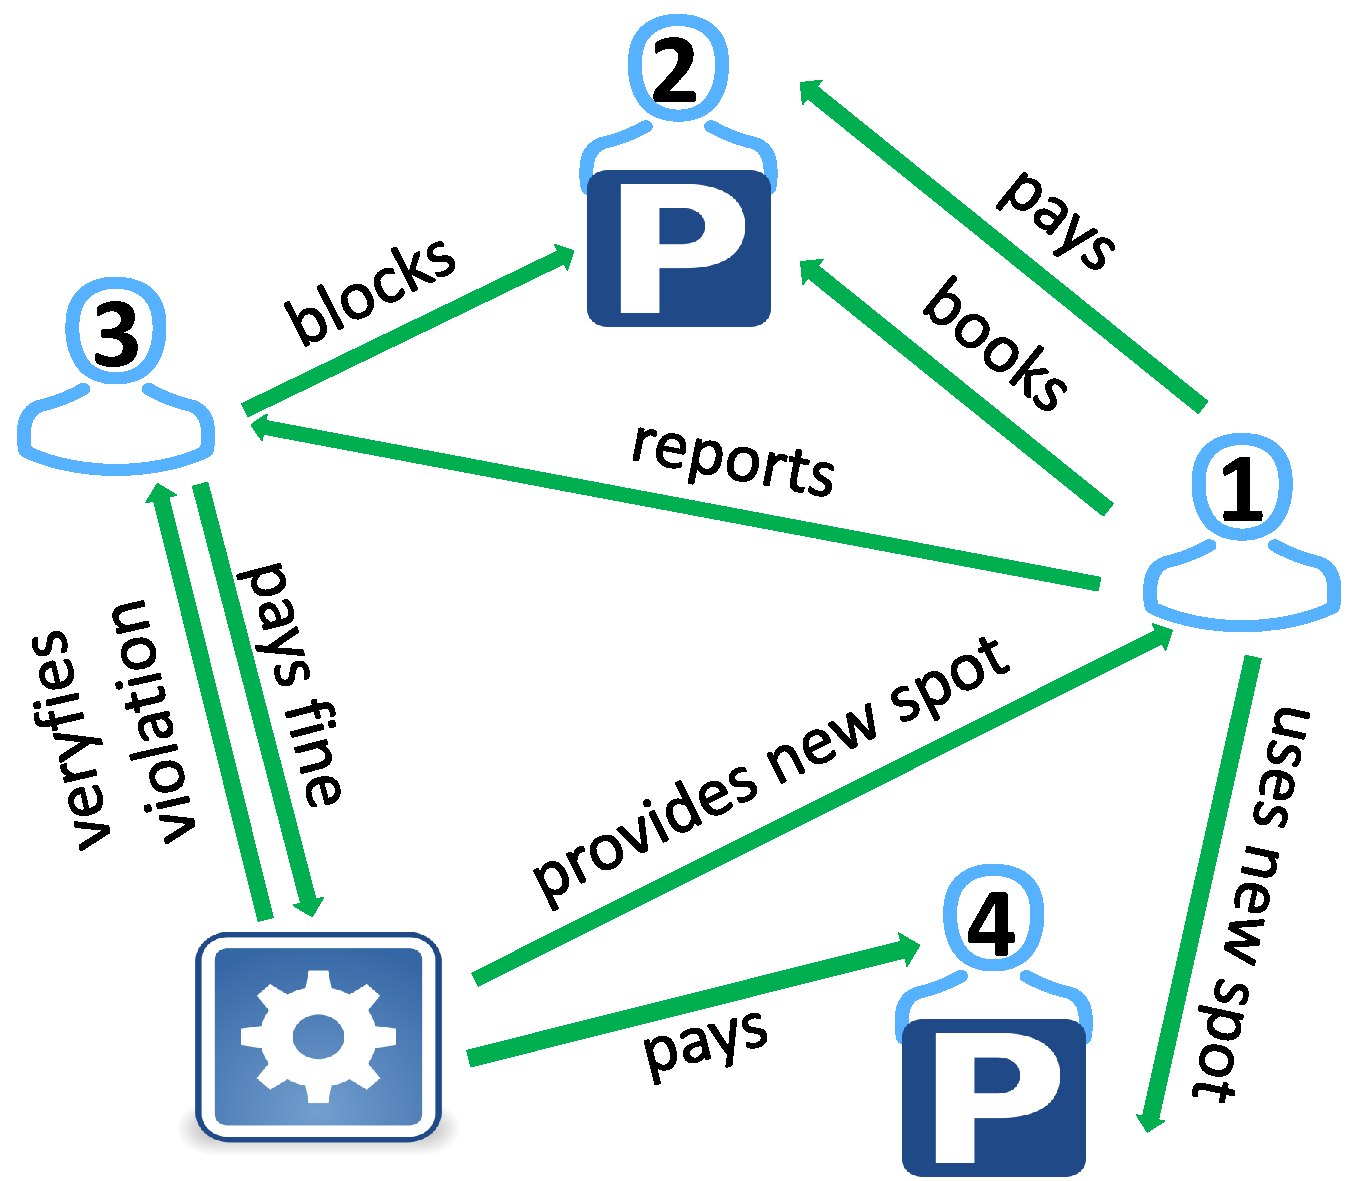
\includegraphics[width=13cm,height=11cm]{example_grafik.pdf}
	\caption{A possible example for the handling of rule violations}
	\label{img:example-grafik}
\end{figure}
 
Of course, it is also conceivable that user 3 has not occupied the parking space at all, but user 1 still reports him. In this case, the verifiers will report that the parking space is actually free. Now the system penalizes user 1 with a sum that covers the costs for the newly allocated parking space (of user 4) and the costs for the verifying users.\\

Another possibility is that user 3 has actually occupied the parking lot but has already left until the users arrive for verification. In this case, like above, the system would identify user 1 as the scammer, although user 3 violated the rules. It also imposes the fine on User 1. He now has the opportunity to challenge the fine. If he does, the confidence score comes into play. If both users are new users or neither of them has a particularly bad or good score, no fair decision can really be made and the costs incurred are borne by the system. In all other cases, when one user is clearly more trustworthy than another, the system decides in favour of the more trustworthy user.


\section{Security Analysis}
In the following, the design of the system is evaluated using the security features set up in the requirement analysis. We look at each point individually. But first we will note a few premise that we believe apply to our system. They will help us perform the security analysis.

\subparagraph{Extensive system} We assume that our system has a large supply and demand. One reason for this is that it is more attractive than other systems, for example because you are compensated as an injured party. Other aspects that can be implemented to achieve this are discussed in the section 'Implementation'.

\subparagraph{Sufficient inspectors} We assume that there are always sufficient inspectors available. The system will be used in places where there are too many cars but too few parking spaces, i.e. in areas with a high population density. As long as the bonus credit for inspectors is reasonably fair, there will always be enough users to do it. In addition, you don't even have to use the app yourself to participate as an inspector. An example of this would be a student who only travels by bicycle but would like to earn a few euros here and there.

\subparagraph{Sufficient parking spaces} We assume that there are always enough parking spaces available for compensation. If the system has low occupancy levels, a suitable free parking space can always be found. If this is not the case, there will always be landlords in larger systems who offer their parking spaces for a particularly expensive price. These places will still be vacant even in situations where almost all capacities are occupied. These are parking spaces that are still available for use as compensation for injured parties, even when there is a high level of occupancy. 

\subparagraph{Fraud is an exception} We assume that fraud in our system is an exception and that most actions are carried out according to the rules. One reason for this is that the majority of people are genuine, especially when they know that offences are being punished hard. We also offer an opportunity to report inadvertent misdemeanours by yourself, in order to prevent major penalties. This also prevents inadvertent misdemeanors by genuine users.\\

Without established data and numbers on fraud in our system, we cannot work with probabilities or the like to show that our design meets the specified requirements. As far as possible, we will therefore work without such data. In places where this is no longer sufficient, we will show that the error probability of our methods approaches 0 with increasing size of the system.

\subsection{Fraud Detection}
Fraud detection includes the simple recognition of fraud as well as the ability to correctly identify the scammer.  \\

Fraud recognition is exclusively achieved by the report system. As soon as a user detects a rule violation, he can report it and the system is informed. It is sufficient to recognize fraud by which another party would be harmed, because this would not be any different without the Shared Parking System. A parking offence only causes problems if another user, who is authorized to park, wants to park on it and with our system the other user now has the ability to report it. Thus, parking spaces with a shared parking system always provide a better possibility for fraud detection than without it. \\

The ability to correctly identify the fraudster is provided by the verification and reputations system. 

\textbf{The following is still early work in progress.}

First, we show that in most cases the verification system alone is sufficient to identify the fraudster.

In order to identify a scammer who illegally occupies a car park (class 1 fraud), it is sufficient that one inspector proves that this user is parked in the parking space. Since we assume an extensive system with sufficient inspectors, the first inspectors can be at the site of the event within minutes. It is unlikely that the scammer will leave the parking lot by then. \\

We show that an genuine user is not identified by the system as a fraudster.

Since we have no fixed figures and data to calculate, we can only estimate that it is very unlikely that the above will occur. Each user starts with the reputation value'neutral'. 


\subsection{Fraud Punishment}
The ability of fraud punishment is based on the ability of fraud detection. If a scammer is correctly identified, the system is able to penalize him. By registering, users have agreed to the rules of the system and can therefore be fined if they violate those rules. In the simplest case, the system receives the money by deducting it from the offender's credit balance and adding it to the system's credit balance. It is therefore obvious that the system receives the entire penalty and can use it for other purposes. If the scammer's credit balance becomes negative through deduction and is not recharged within a certain period of time, the operator receives the penalty in the form of an invoice for contractual penalty to the user.

\subsection{Fraud Prevention}
The system achieves fraud prevention through two methods. On the one hand, scammers are deterred and on the other hand, fraud is uncovered and scammers are thus eliminated.

Scammers are deterred by the public rating system and the well-known possibility of reporting. Anyone who intends to cheat considers twice whether they want to accept the resulting disadvantages, such as a poor rating or exclusion from the system. In addition, there is the fine you have to pay if you are discovered to be a scammer. Since these fines are invariably higher than the cost of using the system properly, fraud is not profitable.

As explained in the paragraph 'Fraud Dedection', scammers are discovered at the latest in the long run. On one hand, all other users notice from the scammer's rating that there is something wrong. The scammer is thus eliminated by the fact that nobody wants to book a parking space of his any more and he will no longer be able to book a parking space from users with manual confirmation, because most users only conclude contracts with users from whom they assume that everything will go as planned, i.e. users with a good rating. On the other hand, scammers are eliminated because they are excluded by the system. Anyone who has been discovered too often as a scammer or whose reputation score falls below a certain threshold will be banned.

\subsection{Fraud Compensation}
Also, fraud compensation can easily be performed once the system has the ability of correctly identifying the fraudster. Further up we have shown that the system has this ability. Once the fraudster has been clearly identified, it is also clear that the other party to the conflict is the injured party which must be compensated. \\

But even before this is clear, the reporting user was provided with a new parking space if required. The costs are initially borne by the system. However, once fraudsters and injured parties have been assigned, the system will recover these costs, as shown in the'Fraud Punishment' section. This means that there are no costs for the system if the scammer can be clearly identified. So if the reporting user was really the injured party, he got a replacement parking space without paying anything for it; he was compensated. If the reporting user was the scammer, however, he had to pay a fine afterwards, meaning that he paid for his replacement parking space by himself.


\section{Implementation}
The system is implemented according to the client-server model. Users utilize a smart phone as a client, while the operator provides a server on which a central database is hosted. Also running on the server is a web service that can be requested by the clients via a REST API. The web sercive forwards the request to the database system and also returns the response back to the clients. An Android app was developed for the clients using Java. The web service is also written in Java and runs on a Tomcat server, while a MySQL server has been set up for the database system.

\section{Future Work}

\section{Conclusion}

\section{Acknowledgments}
I would like to thank Prof. Dr. Alexandra Dmitrienko and the city of Würzburg, who both supported me in creating this work.















%%%
%%% end main document
%%%
%%%%%%%%%%%%%%%%%%%%%%%%%%%%%%%%%%%%%%%%%%%%%%%%%%%%%%%%%%%%%%%%%%%%%%%%%%%%%%%%

% \appendix  %% include it, if something (bibliography, index, ...) follows below

%%%%%%%%%%%%%%%%%%%%%%%%%%%%%%%%%%%%%%%%%%%%%%%%%%%%%%%%%%%%%%%%%%%%%%%%%%%%%%%%
%%%
%%% bibliography
%%%
%%% available styles: abbrv, acm, alpha, apalike, ieeetr, plain, siam, unsrt
%%%
\bibliographystyle{plain}

%%% name of the bibliography file without .bib
%%% e.g.: literatur.bib -> \bibliography{literatur}
\bibliography{thesis}
%\printbibliography[heading=head]

\end{document}
%%% }}}
%%% END OF FILE
%%%%%%%%%%%%%%%%%%%%%%%%%%%%%%%%%%%%%%%%%%%%%%%%%%%%%%%%%%%%%%%%%%%%%%%%%%%%%%%%
%%% Notice!
%%% This file uses the outline-mode of emacs and the foldmethod of Vim.
%%% Press 'zi' to unfold the file in Vim.
%%% See ':help folding' for more information.
%%%%%%%%%%%%%%%%%%%%%%%%%%%%%%%%%%%%%%%%%%%%%%%%%%%%%%%%%%%%%%%%%%%%%%%%%%%%%%%%
%% Local Variables:
%% mode: outline-minor
%% OPToutline-regexp: "%% .*"
%% OPTeval: (hide-body)
%% emerge-set-combine-versions-template: "%a\n%b\n"
%% End:
%% vim:foldmethod=marker
